\documentclass{ppgeesa}

\usepackage[hidelinks]{hyperref}
\usepackage{url}
\usepackage{breakurl}

\usepackage[detect-weight,detect-family]{siunitx}
\sisetup{output-decimal-marker = {,}}
\sisetup{exponent-product = {\cdot}}

\usepackage{Math}
\mathtoolsset{showonlyrefs}
\usepackage{resizegather}
\usepackage{icomma}
\renewcommand{\Prod}{\,}

\usepackage{Figure}
\graphicspath{{../img/}}

\usepackage[inline]{enumitem}

% siunitx % cspell:disable-line
\DeclareSIUnit{\med}{med}
\DeclareSIUnit{\day}{dia}

\begin{document}
\bstctlcite{IEEEBST:Brazilian}

\title{Identificação de Sistema Linear por Erro de Predição}
\author{Guilherme de Paoli Beal
  \\
  {\small Universidade Federal do Rio Grande do Sul}
  \thanks{G. Beal, guilherme.beal@ufrgs.br}
}
\maketitle
\thispagestyle{empty}\pagestyle{empty}

\begin{abstract}
  Aqui vai o resumo.
\end{abstract}

\begin{IEEEkeywords}
  Identificação, Sistema Linear
\end{IEEEkeywords}

\section{Introdução}

O código desenvolvido para este projeto está publicado em \href{https://github.com/GuiBeal/system-identification}{\texttt{github.com/GuiBeal/system-identification}}.

\section{Dados}

Os dados são apresentados na Figura \ref{fig:data}.

\begin{figure}[!htbp]
  \centering
  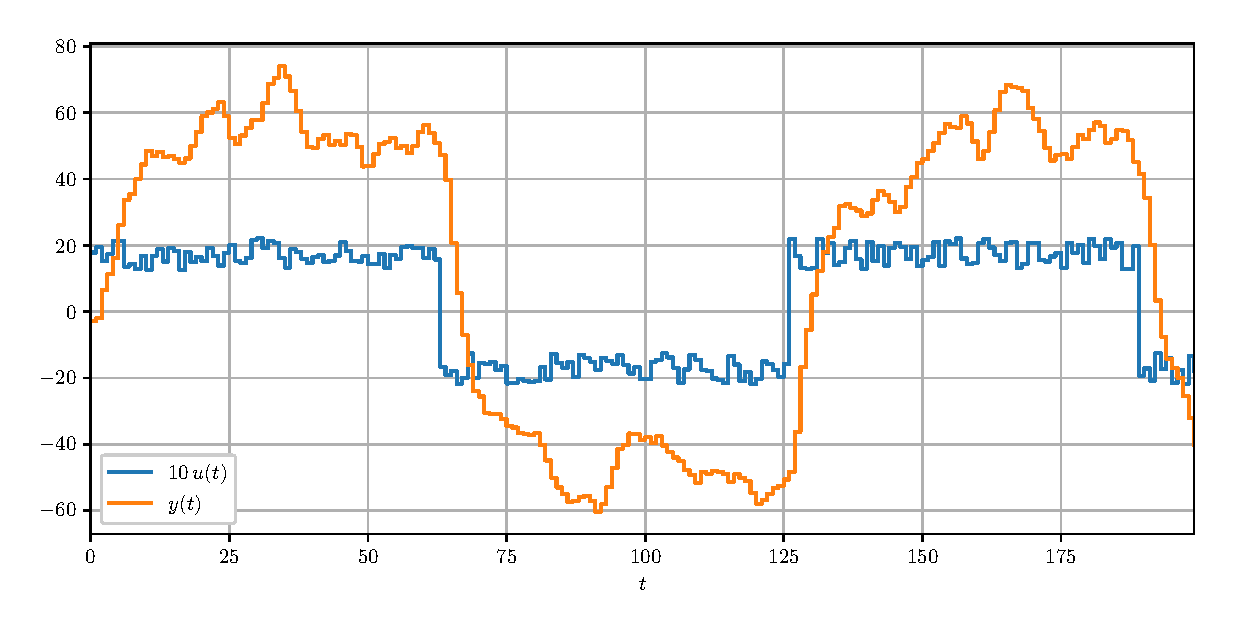
\includegraphics[width=\linewidth]{data}
  \caption{Dados de entrada e saída.}
  \label{fig:data}
\end{figure}

\section{Modelos}

O modelo genérico é representado por
\begin{equation}\label{eq:model}
  A(q) \Prod y[k] = \dfrac{B(q)}{F(q)} \Prod u[k] + \dfrac{C(q)}{D(q)} \Prod e[k]
  ,
\end{equation}
cujos polinômios têm os formatos
\begin{align}
  A(q) &= 1 + a_1 \Prod q^{-1} + \dotsb + a_{n_a} \Prod q^{-n_a}
  ,
  \\
  B(q) &= q^{-n_k} \Prod \left(b_0 + b_1 \Prod q^{-1} + \dotsb + b_{n_b} \Prod q^{-n_b}\right)
  ,
  \\
  C(q) &= 1 + c_1 \Prod q^{-1} + \dotsb + c_{n_c} \Prod q^{-n_c}
  ,
  \\
  D(q) &= 1 + d_1 \Prod q^{-1} + \dotsb + d_{n_d} \Prod q^{-n_d}
  , \text{ e}
  \\
  F(q) &= 1 + f_1 \Prod q^{-1} + \dotsb + f_{n_f} \Prod q^{-n_f}
  ,
\end{align}
em que $n_a$, $n_b$, $n_c$, $n_d$ e $n_f$ são as ordens dos polinômios e $n_k$ é o número de atrasos da entrada para a saída.
Definindo as funções de transferência
\begin{align}
  G(q) &= \dfrac{B(q)}{A(q) \Prod F(q)}
  , \text{ e}
  \\
  H(q) &= \dfrac{C(q)}{A(q) \Prod D(q)}
  ,
\end{align}
então \eqref{eq:model} pode ser reescrita como
\begin{equation}\label{eq:model-tf}
  y[k] = G(q) \Prod u[k] + H(q) \Prod e[k]
  .
\end{equation}

\section{Resultados}

\begin{table}[!htbp]
  \centering
  \caption{Modelos ARX melhor classificados.}
  \begin{tabular}{|c|c|c|c|}
    \hline
    \# & $n_a$ & $n_b$ & $n_k$ \\\hline\hline
    \\\hline
  \end{tabular}
  \label{tab:arx}
\end{table}
\section{Conclusões}

% \bibliographystyle{IEEEtran}
% \bibliography{articles,books,electronic,controlIEEE}

\end{document}
